This chapter describes our approach for generating Puzzle Script levels using different methodologies. Based on the output we conducted our research for generating Puzzle Script rules. This chapter is divided mainly into two parts Level Generation conducted by Rule Generation.

\section{Level Generation}
General Level Generation is not an easy task specially if the main rules can differ from one game. Most of previous work in Puzzle Level Generation (refer to \chref{Chapter3}) was limited for generating levels for a specific game, while the rest just suggest a general technique to be used that is based on designing a game specific fitness function. In this work, we suggest some global metrics for Puzzle Games that can help in generating levels with minimum prior knowledge.\\\par

Our approach relies heavily on the current game rules and objects, and a minimum amount of prior knowledge about Puzzle Script language. \figref{levelGenBlockDiagram} shows a high level block diagram of the system. The following subsections will describe each block in details.

\gfigure{High level system block diagram}{levelGenBlockDiagram}{width=5.5in}{Images/levelGenBlockDiagram}

The system starts by analyzing the current game rules using the Rule Analyzer module. Rule Analyzer module utilize some basic information about Puzzle Script rules to understand the importance of each game object and its basic functionality. Each object is assigned:
\begin{itemize} \itemsep0pt \parskip0pt \parsep0pt
	\item a type
	\item a subtype
	\item a priority within the subtype
	\item a minimum number of objects
	\item a group of behaviors
	\item relations with all other objects
\end{itemize}

The output of the Rule Analyzer and the Level Outlines are fed to Level Generator module. Level Generator is responsible for generating initial level layouts. It utilizes the output of the Rule Analyzer to insert every game objects at a suitable position in the Level Outlines. Level Generator uses two different approaches: Constructive Approach and Genetic Approach. Constructive Approach is faster in generation but produce less diverse levels, while Genetic Approach requires more time but give access to a vast majority of levels.\\\par

The generated levels are subjected to a Level Evaluator module. Level Evaluator uses an automated player to play the generated levels. Based on the result of each play, Level Evaluator gives a score for the level based on six different heuristic measures. These measures make sure the resulting level is playable and not trivial.\\\par

In case of Constructive Approach, the system selects the best scored levels to output them, while Genetic Approach, the system enhances the output levels using GA operators.

\subsection{Rule Analyzer}
Rule Analyzer is the first module in the system. 

\subsection{Level Generator}
\subsubsection{Constructive Approach}
\subsubsection{Genetic Approach}
\textbf{Initial Population:}\\\\
\textbf{Chromosome Representation:}
\subsection{Level Evaluator}
Level Evaluator is responsible for evaluating the generated levels. Evaluating Puzzle Games are based on some heuristic measures. Heuristic measures are based on global knowledge about Puzzle Script games. The first idea was to ensure game playability. That is achieved by using an automated player which we are gonna discuss it later. \figref{diffLevelsSokoban} shows several levels designed for Sokoban game where all are playable but some of them are more interesting than other. The first level is very easy level which can be solve with one move. The second level need more moves which is more interesting than the first level but it is just straight forward toward the solution. The last level is not easy to solve need some prior thinking and trying some moves which is more interesting than previous two.

\gfigure{Examples on different levels for Sokoban game}{diffLevelsSokoban}{width=5.5in}{Images/diffLevelsSokoban}

The above example proves that playability is not enough to judge puzzle levels. Some other metrics must be used to ensure the solution have more moves with some thinking ahead. Six heuristics measures are applied on the output of the automated player to capture this feature.

\subsubsection{Automated Player}
Our Level Evaluator uses a modified version of the BestFS Algorithm as automated player. BestFS Algorithm was introduced in Lim et al.\cite{puzzleScriptGeneration} work. BestFS is similar to BFS algorithm but instead of exploring states sequentially, it sorts them according to fitness function. This causes the algorithm to explore the more important nodes first helping it to reach the solution faster. As explained in \chref{Chapter3}, Lim et al. algorithm uses two metrics to evaluate each game state:
\begin{itemize} \itemsep0pt \parskip0pt \parsep0pt
	\item \textbf{Distance between winning objects:} BestFS tries to either increase or decrease the distance between the winning objects according to the winning rule. The "No" rule is the only rule that need to increase the distance, while the others need to decrease it. \figref{bestFS1} shows an example from Sokoban, where the distance between crates and targets is highlighted.
	\item \textbf{Distance between player and winning objects:} BestFS always tries to minimize the distance between the player and the winning objects. In order to affect the distance between the winning objects, player should come near toward them. \figref{bestFS2} shows same level from Sokoban, where the distance between player and winning objects (crates and targets) is highlighted.
\end{itemize}

\begin{hcfigure}
	\centering
	\begin{minipage}{0.45\textwidth}
		\centering
  		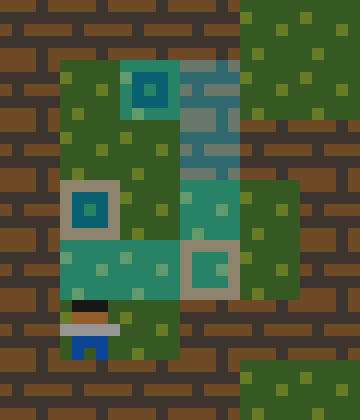
\includegraphics[width=\linewidth]{Images/firstScoreBestFS}
  		\caption{Example of distance between winning objects metric}\label{Figure:bestFS1}
	\end{minipage}\hfill
	\begin{minipage}{0.45\textwidth}
		\centering
  		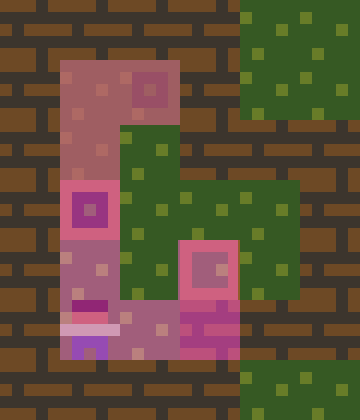
\includegraphics[width=\linewidth]{Images/secondScoreBestFS}
  		\caption{Example of distance between player and winning objects metric}\label{Figure:bestFS2}
	\end{minipage}
\end{hcfigure}

That metric works fine for all games where player is not one of the winning objects. In that case, the two metrics behaves in the same way so the player always try to move towards goal regardless of other game objects. For example, \figref{lavaGame} shows a level from a game called LavaGame. LavaGame is a puzzle game where the goal is to make the player reaches the exit. The path to the exit is usually stuck by lava which can be destroyed by pushing a crate over it. According to the metrics, the player will try to move nearer to the exit by either going left. These movement will not help him to reach the goal, so the player will start wandering aimlessly trying to stumble about a sequence help him reach the goal.

\gfigure{Example level from LavaGame showing the problem in the old metrics}{lavaGame}{width=3.0in}{Images/lavaGame}

Player's aim is to move crates towards lava to unblock his path towards the exit. This aim is somehow explained in the game rules, so by further analysis the game rules we can know which objects need to be closer. Returning to our example about LavaGame, the game rules are stated in the following order:
\begin{center}{[> Player | Crate] -> [> Player | > Crate]}\end{center}
\begin{center}{[> Crate | Lava] -> [ \ \ \ \ | \ \ \ \ ]}\end{center}
The first rule says if there is a player and crate beside each other and the player moves toward it, the crate will also move. The second rule says if there is a crate and lava beside each other and the crate moves toward it, both crate and lava will be destroyed. In any proper game, rules must be applied before achieving the winning condition. Based on that fact, the distance between objects on the left hand side of the rules must be decreased. The new heuristic is the distance between objects in the left hand side of the rules. The relation between objects in the left hand side of the rules is captured by the Rule Analyzer module.\\\par

The three metrics are weighted with respect to each other and used as a new function to evaluate each game state. The weights are chosen by experimentation to ensure best results. The automated player returns four different values that are analyzed and used in the Heuristic measures in the next section. These four values are:
\begin{itemize} \itemsep0pt \parskip0pt \parsep0pt
	\item The score for the best reached state so far. The score is calculated using the first metric (Distance between winning objects). The score value is in range between [0, 1], where the score is equal 1 when a solution is found.
	\item The sequence of movements to reach the best state. The automated player saves up all the movement happens to reach each state.
	\item The number of states explored while searching for the solutions. The automated player increment a variable whenever it explore a new state.
	\item The number of rules that the game engine applied to reach the best state. The game engine increment a variable whenever any of the game rules is applied.
\end{itemize}
The modified BestFS find solution faster than before. More details will be expressed in \chref{Chapter5}.\\\par

\subsubsection{Heuristic Measures}
Heuristic Measure are calculated using a weighted function of six attributes. The function is described as the following:
\begin{center}$F_{score} = 0.3 * P_{score} + 0.2 * L_{score} + 0.15 * N_{score} + 0.12 * B_{score} + 0.12 * R_{score} + 0.11 * E_{score}$\end{center}
where $P_{score}$ is Playing Score, $L_{score}$ is Solution Length Score, $N_{score}$ is Object Number Score, $B_{score}$ is Box Line Score, $R_{score}$ is Applied Rule Score, and $E_{score}$ is Exploration Score. The weights for each attribute are measured experimentally to reflect the importance of some features with respect to the others.\\\\
\textbf{Playing Score ($P_{score}$):} Playing score is used to ensure playability of the level. Instead of using a boolean value for playable or not. Score is assigned a value for how much you are near the solution. Automated player is used to play the game and return a value from [0, 1] where 0 means there is no objects at all, while 1 which means the agent reached the solution. Making the domain more continuous helps in measuring the percentage of the level playability. Instead of using it as a constraint to be satisfied.\\\par

Based on the work by Nielsen et al.\cite{gvgpPerformanceProfiles} which proved that Do Nothing player is an important measure for good designed games. A score is calculated for the initial level state and subtracted from the result of the automated player. The heuristic measure can be expressed by the following equation:
\begin{center}$ P_{total} = P_{score} - N_{score}$\end{center}
where $P_{score}$ is the automated player score and $N_{score}$ is the Do Nothing player score.\\\\
\textbf{Solution Length Score ($L_{score}$):} \figref{diffLevelsSokoban} shows that interesting levels usually have more steps than trivial ones. The first idea was to use the length of best movement sequence the automated player has reached and compare it with a required value. This idea will not work as expected because solution length depends on the size of the level. For example, \figref{sokobanLenghtArea} shows different levels from Sokoban and the corresponding solution length. Its obvious that the seconds level have longer solution length than the first one because it have huger area.

\gfigure{Examples of two sokoban levels with different area and solution lengths}{sokobanLenghtArea}{width=4.5in}{Images/sokobanLenghtArea}

From the previous example we can conclude that the solution length depends on the level area. Instead of using the solution length as the metric we used the ratio between the solution length and the level area. A mapping function is need to convert that number to a value in the range [0, 1]. We analyzed 40 hand crafted levels with different area from 5 different games. A histogram is plotted on the collected values of the ratio between the solution length and the level area.

\gfigure{Histogram for the ratio between the solution length and the level area}{solutionLengthHistogram}{width=5.5in}{Images/solutionLengthHistogram}

The histogram in \figref{solutionLengthHistogram} seems to follow a Gaussian Distribution with $\mu = 1.221$ and $\sigma = 0.461$. Based on that, the Solution Length Score is expressed by the following equation:
\begin{center}$L_{score} = Gaussian(\dfrac{L}{A}, 1.221, 0.461)$\end{center}
where $Gaussian(Ratio, \mu, \sigma)$ is a gaussian operator, $L$ is the solution length score, and $A$ is the level area.\\\\
\textbf{Object Number Score ($N_{score}$):} It is divided into 3 parts:
\begin{itemize} \itemsep0pt \parskip0pt \parsep0pt
	\item \textbf{Number of Rule Objects:} In a good designed level, most of the rule objects should appear in the level to ensure there is a possibility of applying each rule. The minimum number of times the object should appear in the level must be greater than or equal his minimum number property from Rule Analyzer.
	\item \textbf{Number of Players:} The game should have only one player. If the level have any other value, this part pf the score will be zero.
	\item \textbf{Number of Winning Objects:} The number of the winning objects should be equal, unless one of the winning objects have "Create" behavior. Based on the previous condition, the score is set either to one or zero.
\end{itemize}
Object Number Score is calculated using the following equation:
\begin{center}$N_{score} = 0.4 * N_{rule} + 0.3 * N_{player} + 0.3 * N_{winning}$\end{center}
where $N_{rule}$ is the Number of Rule Objects, $N_{player}$ is the Number of Players, and $N_{winning}$ is the Number of Winning Objects.\\\\
\textbf{Box Line Score ($B_{score}$):} It is similar to Taylor and Parberry\cite{sokobanLevelGenerationNew} metric used to find the farthest state. This metric calculates the number of unrepeated moves found in the solution and divide it by total length of the solution. The following equation represents the metric:
\begin{center}$B_{score} = \dfrac{L_{unique}}{L}$\end{center}
where $L_{unique}$ is the number of unrepeated moves in the solution and $L$ is the solution length.\\\\
\textbf{Applied Rule Score ($R_{score}$):} Number of applied rules in the best playing sequence.\\\\
\textbf{Exploration Score ($E_{score}$):} Number of explored states before the best game state.

\section{Rule Generation}
\subsection{Chromosome Representation}
\subsection{Fitness Function}

\tabref{l1}

\tabref{3.1}~demonstrates $\ldots$.

\gtable{Example table for demonstration}{3.1}{width=5.0in}{Table3-1}

\begin{table}
	\label{Table:l1}
	\centering
	\begin{tabular}{|c|c|c|}
		\hline
		xxxx & 1233 & ccccc \\
		\hline
		uuuuu & 2323 & gggggg \\
		\hline
	\end{tabular}
	\caption{Example table for demonstration}
\end{table}

\tabref{3.2}.

\begin{landscape}
\gtable{Another example wide table for demonstration}{3.2}{width=9.0in}{Table3-2}
\end{landscape}